\documentclass[11pt,a4paper]{article}

\usepackage[spanish, es-nodecimaldot]{babel}
\usepackage[T1]{fontenc}
\usepackage[utf8]{inputenc}

% Math essentials
\usepackage{amsmath, amssymb}
\usepackage{bm}

% Units and hyperlinks
\usepackage{siunitx}
\sisetup{per-mode=symbol}

\usepackage{natbib}
\usepackage{graphicx}
\usepackage{lmodern}
\usepackage{caption}
\usepackage{subcaption}
\usepackage{float}
\usepackage{url}
\usepackage{titlepic}
\usepackage{listings}
\usepackage{nameref}
\usepackage{xcolor}
\usepackage{array}
\setlength{\marginparwidth}{2cm}
\usepackage{todonotes}
\usepackage{datetime}
\usepackage{parskip}
\usepackage{hyperref}

% ------- Macros definidas en este documento -------
\newcommand{\vect}[1]{\bm{#1}}       % vectores en negrita cursiva
\newcommand{\mat}[1]{\mathbf{#1}}    % matrices en negrita recta
\newcommand{\trans}{\mathsf{T}}      % traspuesta, usar como ^{\trans}

% \newcommand{\SO}{\mathrm{SO}}
% \newcommand{\SE}{\mathrm{SE}}

\newcommand{\skewsym}[1]{\left[#1\right]_\times}

\newcommand{\SkewFrom}[3]{%
  \begin{bmatrix}
    0 & -#3 & #2 \\
    #3 & 0 & -#1 \\
    -#2 & #1 & 0
  \end{bmatrix}%
}

\title{Cinemática de robots terrestres}
% \author{ \includegraphics[width=0.5\linewidth]{images/logo.jpg} }
\author{Juan Francisco Rascón Crespo}
\date{\today}

\setcounter{secnumdepth}{2}
\setcounter{tocdepth}{2}

\begin{document}
\maketitle

% \thispagestyle{empty}
% \newpage

% \tableofcontents
% \newpage

\section{Restricciones de las ruedas}
\todo[inline]{Completar}

\section{Base con tres ruedas activas orientables (three swerve drive)}
% \subsection{Simulación de los AGVs}
% \label{sec:state-machine}

La base con tres ruedas activas orientables (three swerve drive) es un sistema de locomoción omnidireccional. Permite que un robot terrestre se mueva en cualquier dirección sin tener que cambiar antes la orientación del chasis. Cada rueda se orienta de forma independiente, por lo que el robot gana maniobrabilidad y flexibilidad.

\begin{figure}[H]
    \centering
    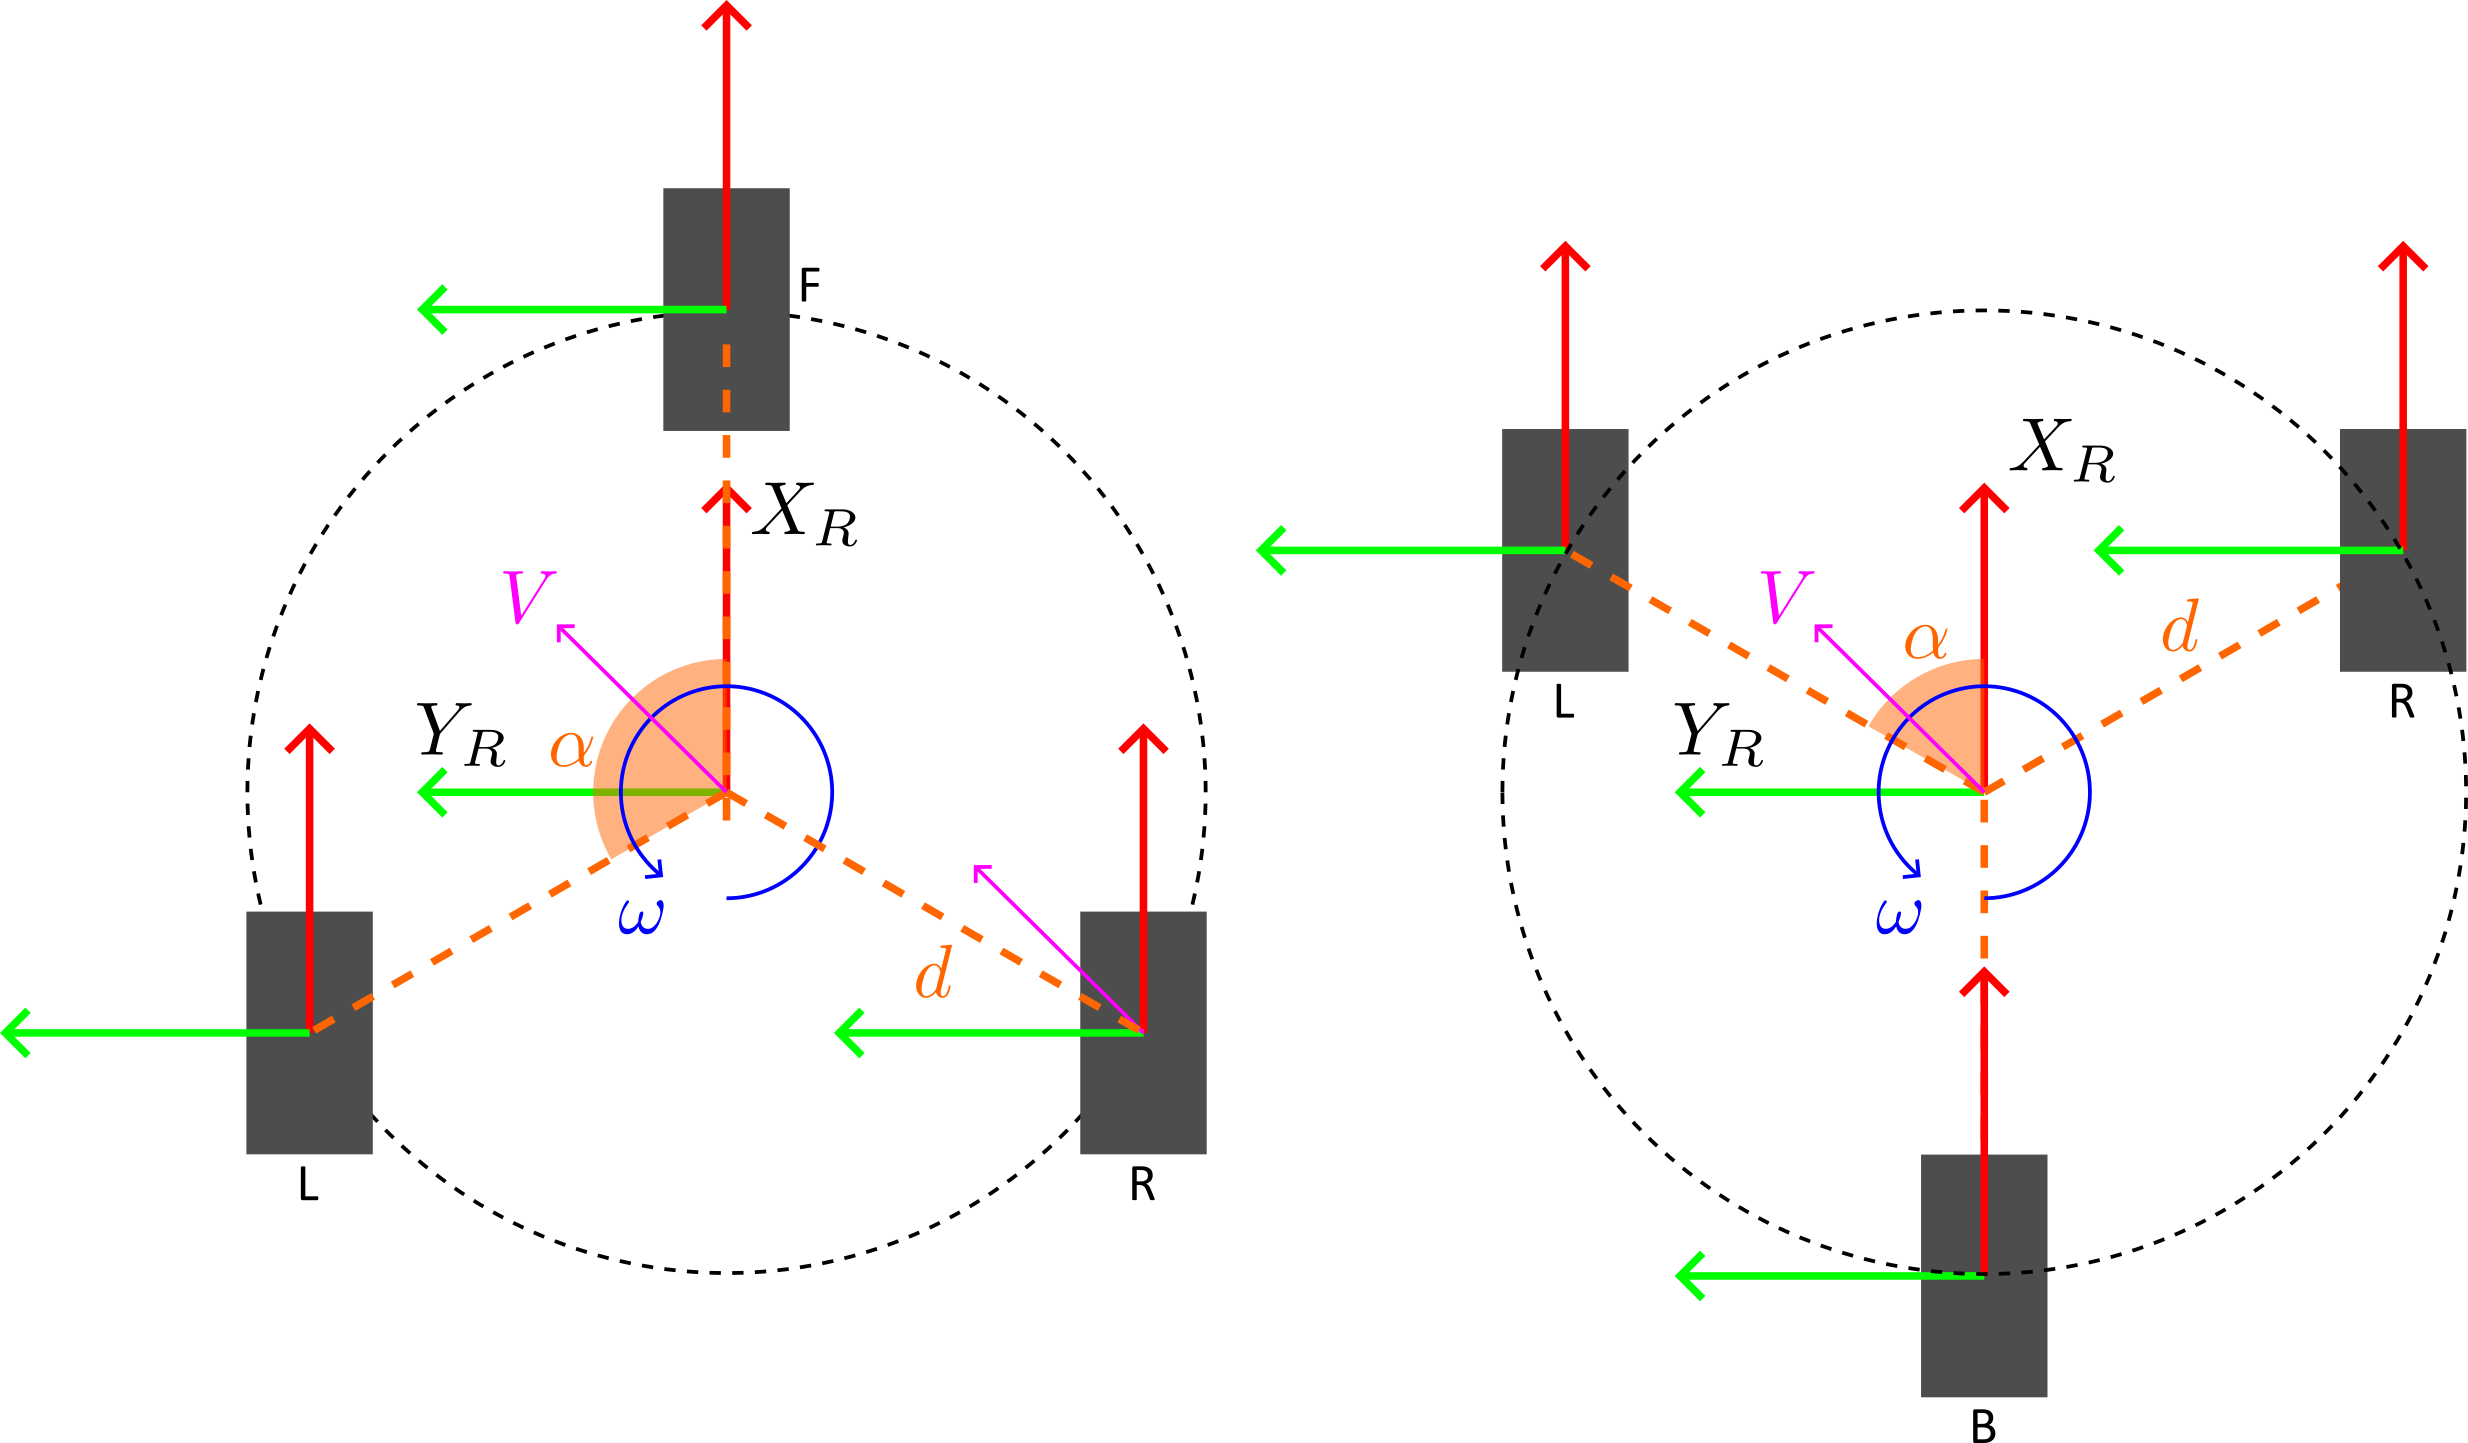
\includegraphics[width=1.0\linewidth]{images/three_drive_configuration.png}
    \caption{Configuraciones comunes de las ruedas en un sistema three swerve drive (izquierda: configuración Y-invertida, derecha: configuración Y)}
    \label{fig:three-swerve-drive-configuration}
\end{figure}

La disposición típica de las ruedas es triangular. Las dos configuraciones más comunes son:

\begin{itemize}
    \item Configuración Y-invertida: Una rueda se coloca a distancia $d$ del centro sobre el eje $X_R$ positivo. Las otras dos se colocan también a distancia $d$, en los ángulos $\alpha^\circ$ y $-\alpha^\circ$ respecto del eje $X_R$ positivo, con $\alpha \in [90^\circ, 180^\circ)$.
    \item Configuración Y: Una rueda se coloca a distancia $d$ del centro sobre el eje $X_R$ negativo. Las otras dos se colocan también a distancia $d$, en los ángulos $\alpha^\circ$ y $-\alpha^\circ$ respecto del eje $X_R$ positivo, con $\alpha \in (0^\circ, 90^\circ]$.
\end{itemize}

La figura \ref{fig:three-swerve-drive-configuration} muestra ambas configuraciones.

A continuación se presentan las expresiones de la cinemática inversa y directa de un robot con tres ruedas activas para las configuraciones anteriores. También puede considerarse una formulación más general, con distancias al centro distintas o con ruedas en ángulos no simétricos. Sin embargo, estas configuraciones son menos frecuentes y, en este contexto, solo complican las expresiones sin aportar ventajas prácticas, ya que, en la industria, se emplean principalmente las configuraciones descritas anteriormente.

Para la configuración Y-invertida, se usará $i \in \{F,L,R\}$ para identificar cada rueda.
Para la configuración Y, se usará $i \in \{B,L,R\}$.

La velocidad lineal de la base se denota como:
\begin{equation}
    \vect{V} = \begin{bmatrix} V_x \\ V_y \\ 0 \end{bmatrix}
    \label{eq:rigid-velocity}
\end{equation}
y se expresa en \si{\meter\per\second}.

La velocidad angular de la base se denota como:
\begin{equation}
    \boldsymbol{\omega} = \begin{bmatrix} 0 \\ 0 \\ \omega_z \end{bmatrix}
    \label{eq:rigid-angular-velocity}
\end{equation}

La velocidad lineal de cada rueda $i$ se expresa como:
\begin{equation}
    \begin{aligned}
        \vect{V}_i & = \vect{V} + \vect{\omega} \times \vect{d}_i           \\
                   & = \vect{V} + \skewsym{\boldsymbol{\omega}}\,\vect{d}_i
    \end{aligned}
    \label{eq:wheel-velocity}
\end{equation}
donde $\vect{d}_i$ es el vector de posición de la rueda $i$ respecto al centro de la base.

El producto vectorial entre $\boldsymbol{\omega}$ y $\vect{d}_i$ puede escribirse como un producto matricial mediante el operador antisimétrico $[\cdot]_{\times}$:
$\boldsymbol{\omega} \times \vect{d}_i = \skewsym{\boldsymbol{\omega}}\,\vect{d}_i$, y
$\skewsym{\boldsymbol{\omega}}$ se define como:
\[
    \skewsym{\boldsymbol{\omega}} \triangleq
    \SkewFrom{\omega_x}{\omega_y}{\omega_z}
\]

Por lo tanto, considerando $\boldsymbol{\omega}=\begin{bmatrix}0&0&\omega_z\end{bmatrix}^{\trans}$ y $\vect{d}_i=\begin{bmatrix}d\cos\alpha_i&d\sin\alpha_i&0\end{bmatrix}^{\trans}$:
\begin{equation}
    \vect{V}_i
    = \vect{V}
    + \begin{bmatrix}
        -\omega_z d\sin\alpha_i \\
        \omega_z d\cos\alpha_i  \\
        0
    \end{bmatrix}
    = \begin{bmatrix}
        V_x - \omega_z d\sin\alpha_i \\
        V_y + \omega_z d\cos\alpha_i \\
        0
    \end{bmatrix}
    \label{eq:wheel-velocity-expanded}
\end{equation}

La magnitud de la velocidad lineal de cada rueda $i$ se expresa como:
\begin{equation}
    \begin{aligned}
        \|\vect{V}_i\| = \sqrt{(V_x - \omega_z d\sin\alpha_i)^2 + (V_y + \omega_z d\cos\alpha_i)^2} = \omega_i r
    \end{aligned}
    \label{eq:wheel-speed}
\end{equation}

donde $r$ es el radio de la rueda y $\omega_i$ es la velocidad angular de la rueda $i$.

Obviamente, todas las ruedas tienen el mismo radio $r$.

\subsection{Cinemática inversa}

Se denomina cinemática inversa al proceso de calcular las velocidades de las ruedas $\omega_i$, y su orientación $\theta_i$, a partir de la velocidad lineal $\vect{V}$ y la velocidad angular $\boldsymbol{\omega}$ de la base.

Se calcula la orientación de cada rueda $i$, $\theta_i$, a partir de su velocidad lineal $\vect{V}_i$:
\begin{equation}
    \theta_i = \arctan2(V_{iy}, V_{ix}) = \arctan2(V_y + \omega_z d\cos\alpha_i, V_x - \omega_z d\sin\alpha_i)
    \label{eq:inverse-kinematics-angle}
\end{equation}

A continuación, se obtiene la velocidad angular de cada rueda $i$, $\omega_i$, a partir de su velocidad lineal, $\vect{V}_i$, y su radio, $r$:
\begin{equation}
    \omega_i = \frac{\|\vect{V}_i\|}{r} = \frac{\sqrt{(V_x - \omega_z d\sin\alpha_i)^2 + (V_y + \omega_z d\cos\alpha_i)^2}}{r}
    \label{eq:inverse-kinematics-speed}
\end{equation}


\begin{figure}[H]
    \centering
    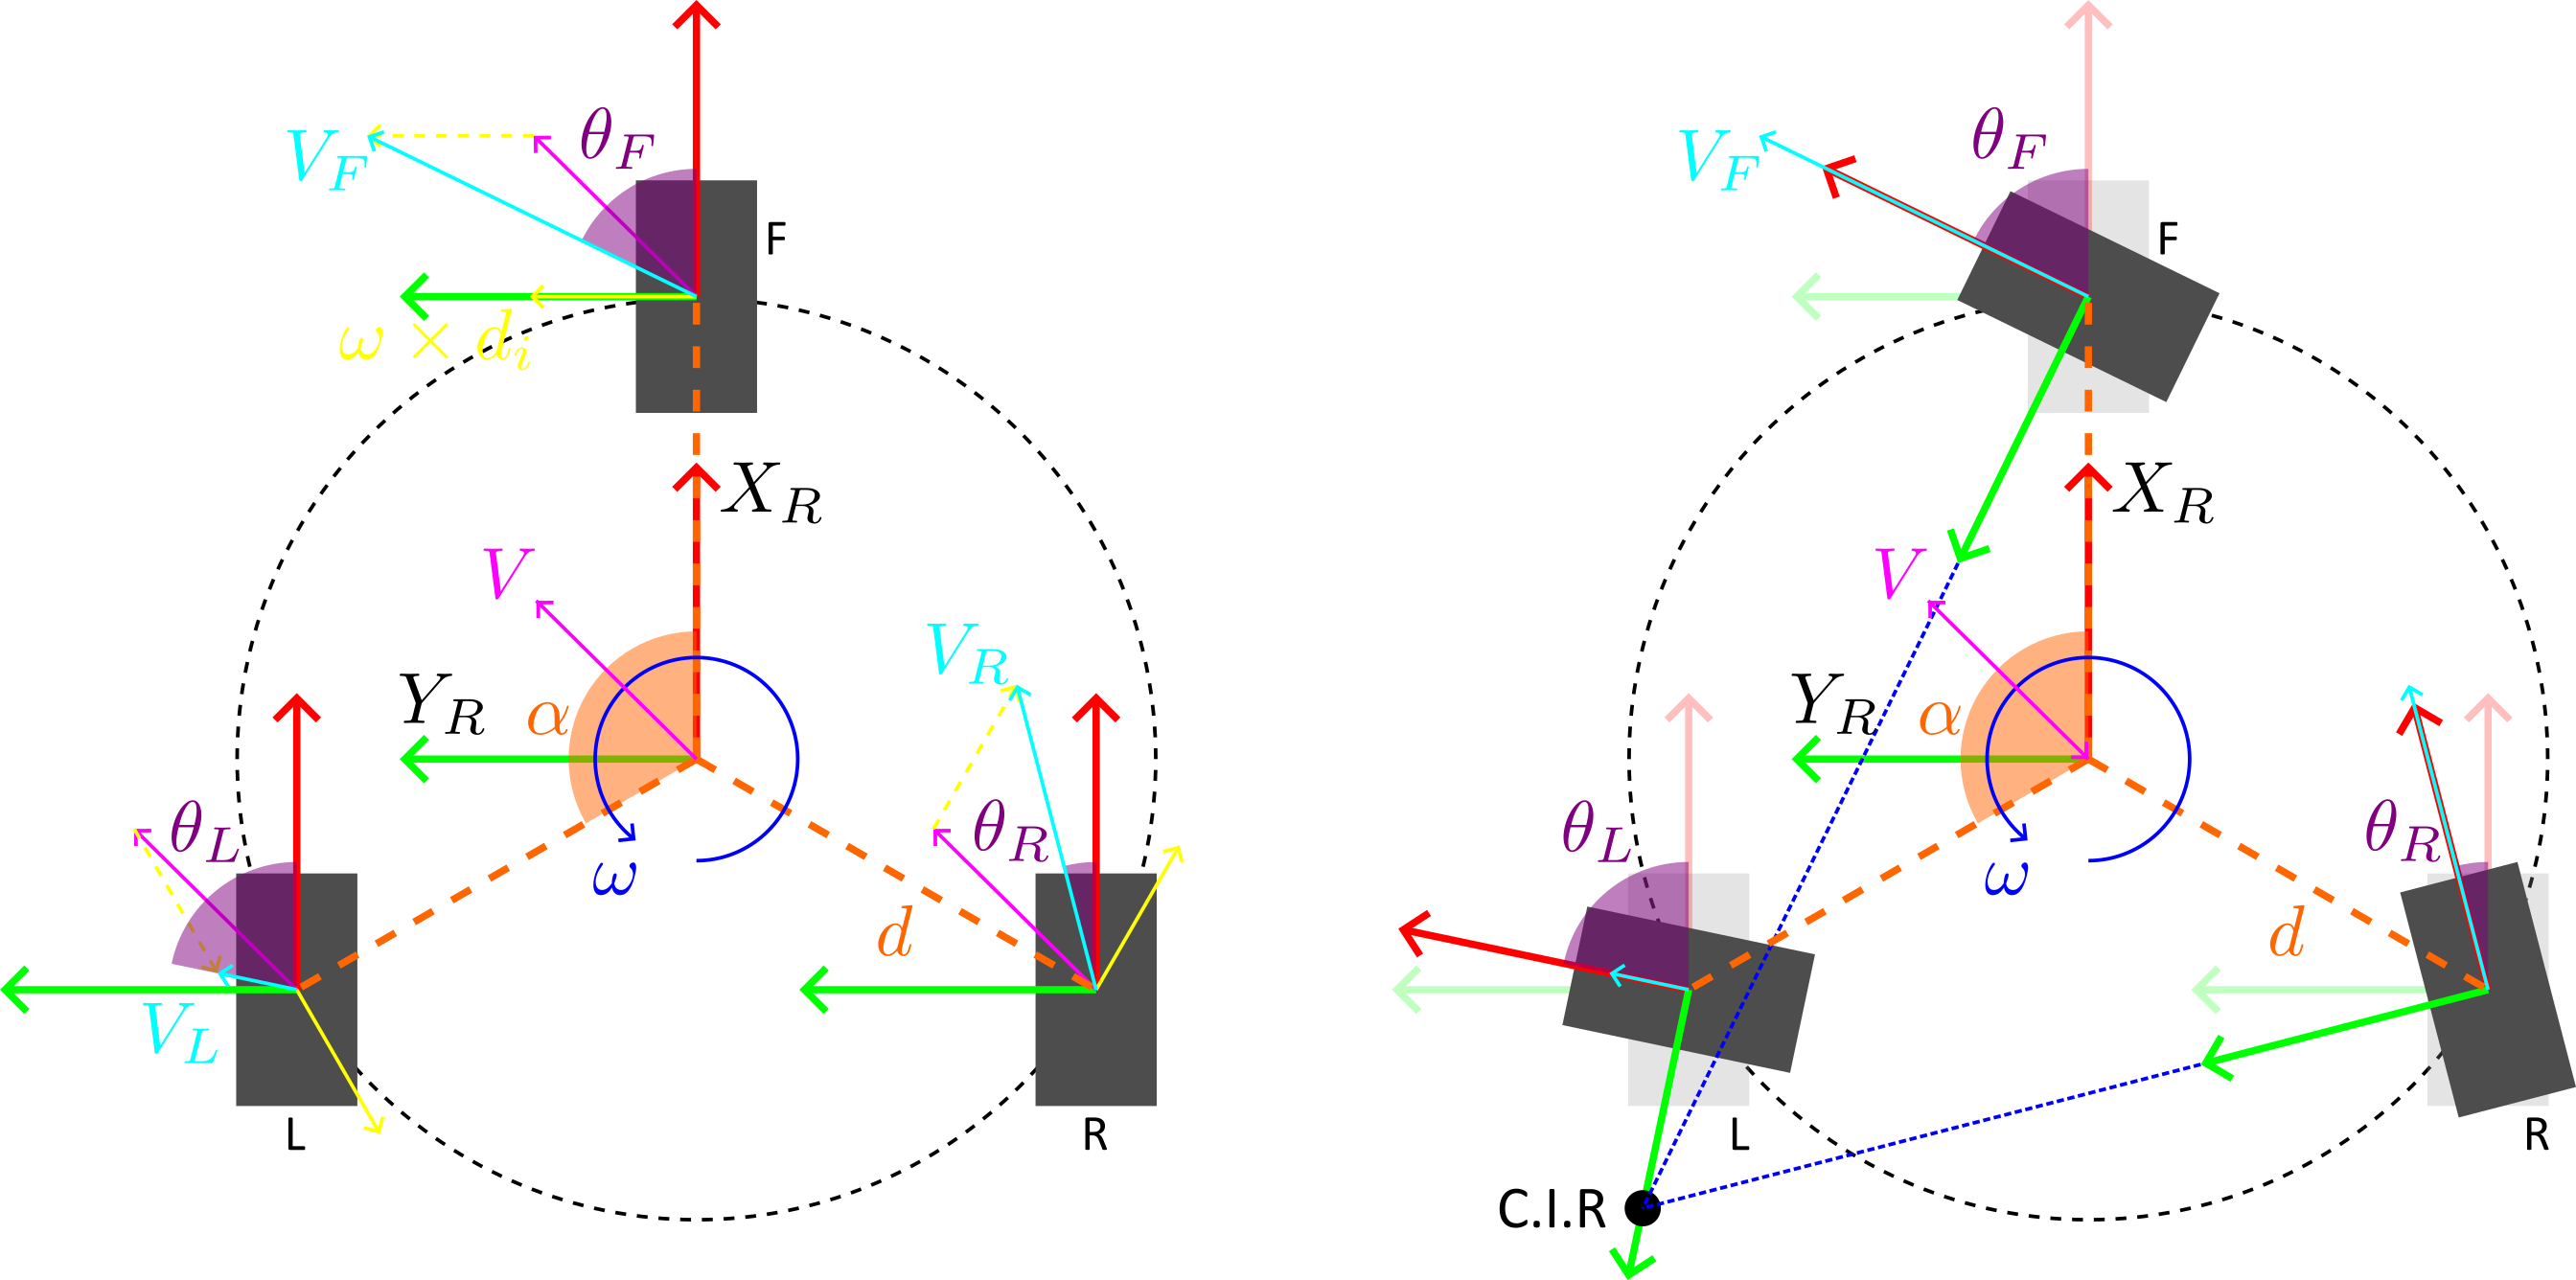
\includegraphics[width=1.0\linewidth]{images/inverted_y_inverse_kinematics.png}
    \caption{Cinemática inversa de un robot con configuración Y-invertida.}
    \label{fig:inverted-y-inverse-kinematics}
\end{figure}

\begin{figure}[H]
    \centering
    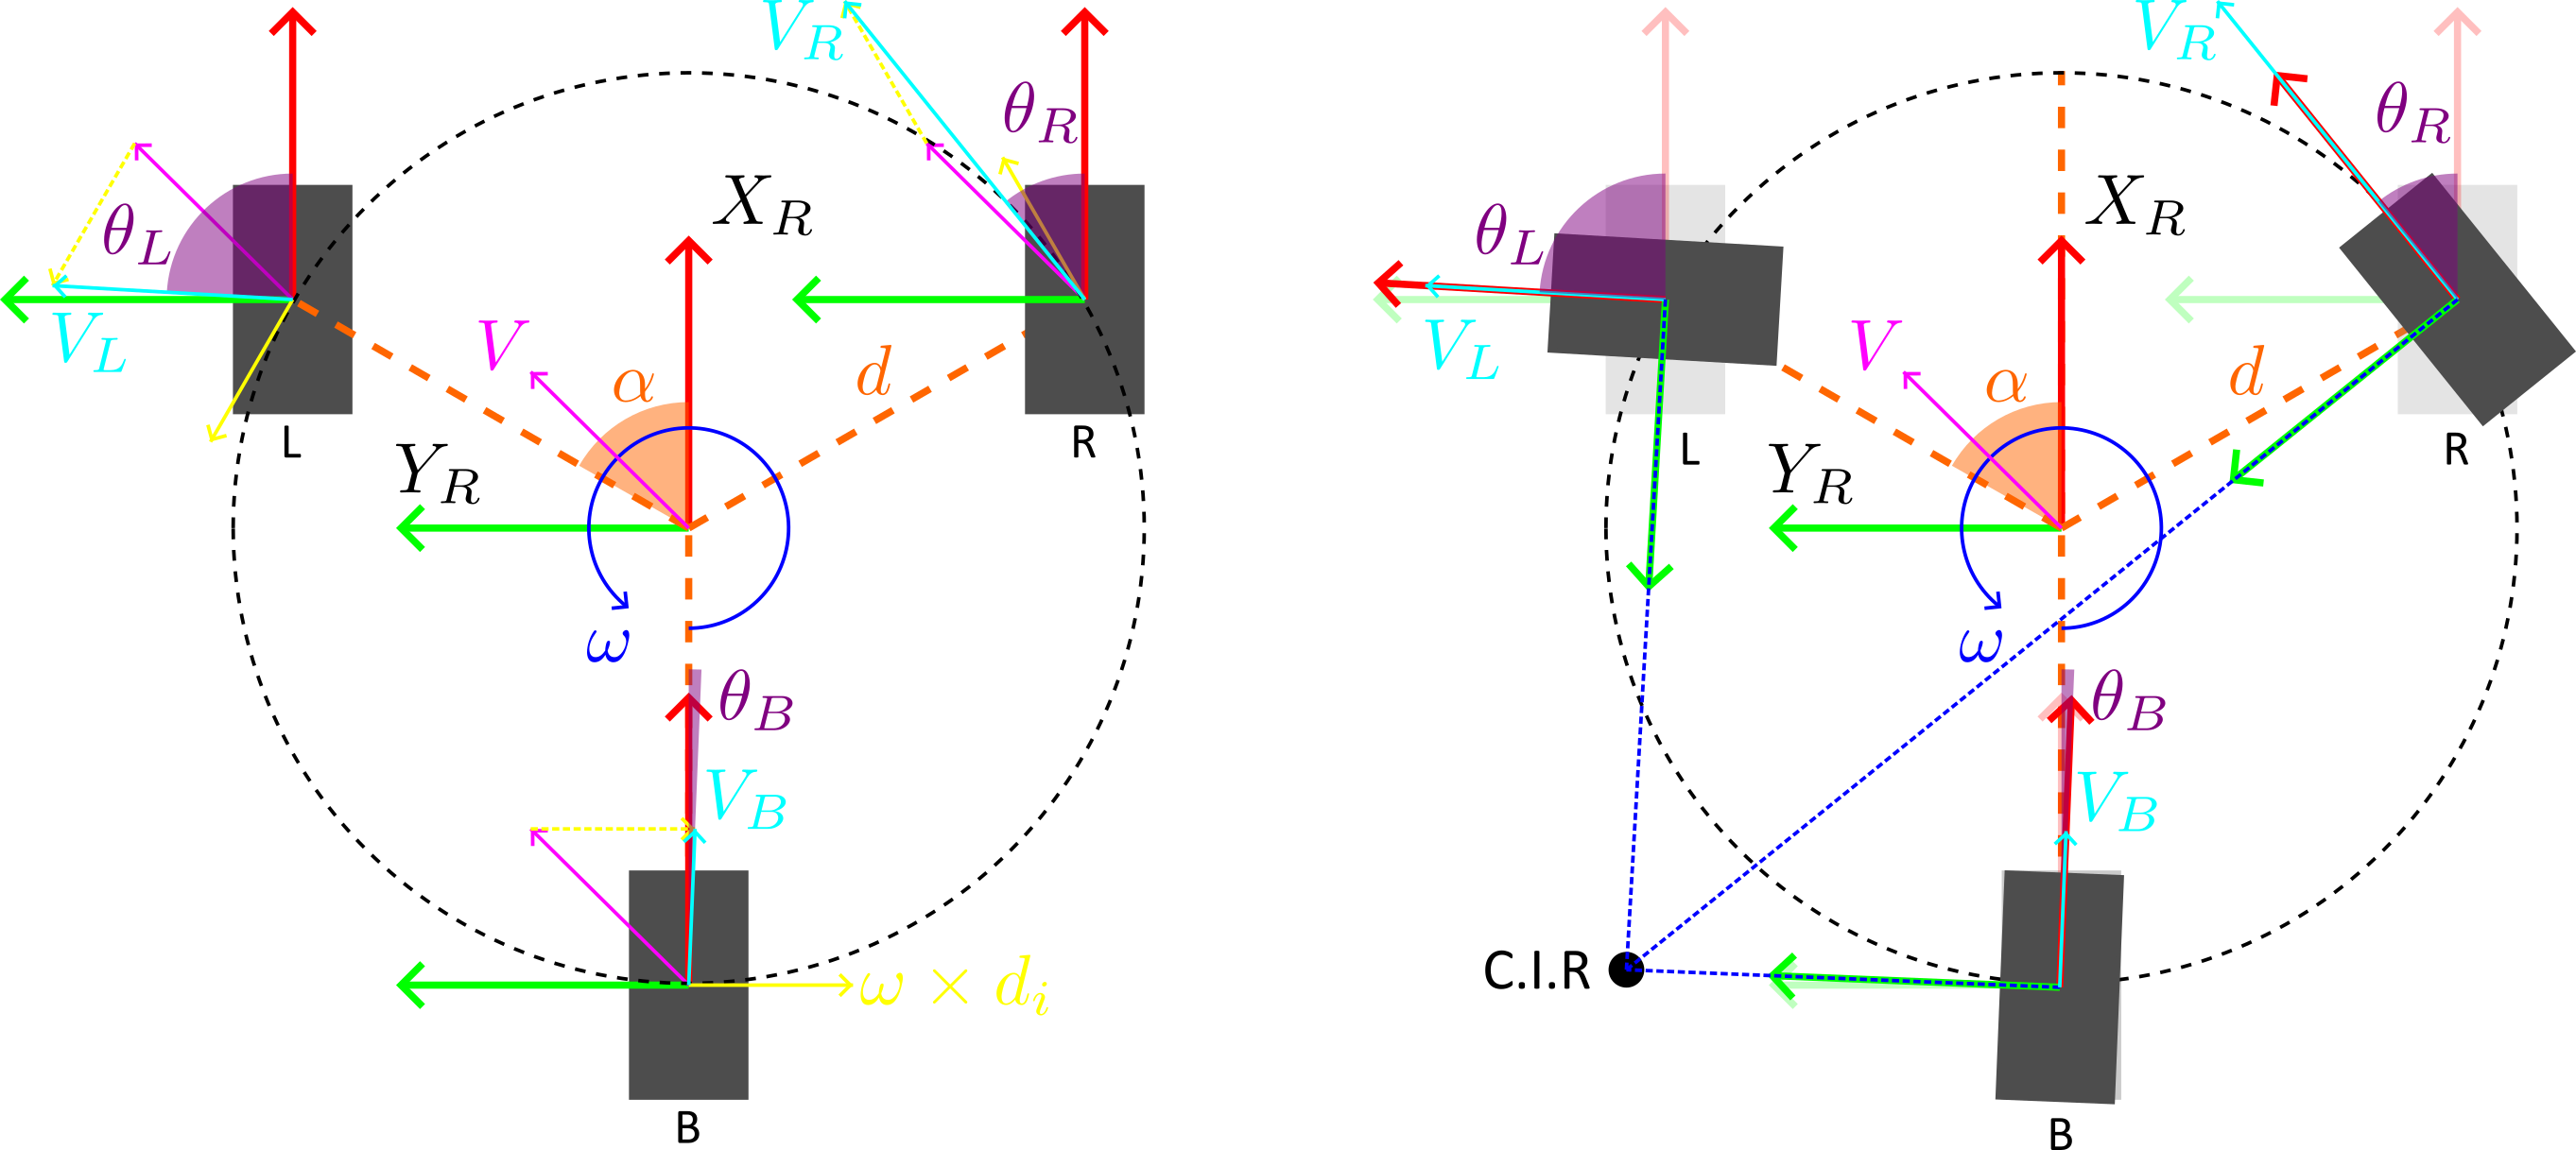
\includegraphics[width=1.0\linewidth]{images/y_inverse_kinematics.png}
    \caption{Cinemática inversa de un robot con configuración Y}
    \label{fig:y-inverse-kinematics}
\end{figure}

\subsection{Cinemática directa}

Se denomina cinemática directa al proceso de calcular la velocidad lineal $\vect{V}$ y la velocidad angular $\boldsymbol{\omega}$ de la base a partir de las velocidades angulares $\omega_i$ y las orientaciones $\theta_i$ de las ruedas.

Se conocen 6 variables de entrada: las velocidades angulares $\omega_i$ y las orientaciones $\theta_i$ de cada rueda $i$. Se desea calcular 3 variables de salida: la velocidad lineal $\vect{V} = (V_x, V_y, 0)^{\mathsf{T}}$ y la velocidad angular $\boldsymbol{\omega} = (0, 0, \omega_z)^{\mathsf{T}}$ de la base. Por lo tanto, el sistema es sobredeterminado y se resuelve de forma robusta mediante mínimos cuadrados.
En la configuración Y-invertida se usa $i \in \{F,L,R\}$ (Front, Left, Right). Para la configuración Y, se sustituye por $i \in \{B,L,R\}$ (Back, Left, Right).

Para cada rueda $i$, se define el vector unitario de rodadura:
\begin{equation}
    \vect{t}_i = \begin{bmatrix}
        \cos\theta_i \\
        \sin\theta_i \\
        0
    \end{bmatrix}
    \label{eq:wheel-rolling-direction}
\end{equation}

La velocidad lineal de la rueda en su dirección de rodadura es:
\begin{equation}
    \vect{V}_i = r\omega_i \vect{t}_i
    = r\omega_i
    \begin{bmatrix}
        \cos\theta_i \\
        \sin\theta_i \\
        0
    \end{bmatrix}
    \label{eq:wheel-linear-from-omega}
\end{equation}

Igualando \eqref{eq:wheel-velocity-expanded} y \eqref{eq:wheel-linear-from-omega}, para cada rueda $i$ se obtiene:
\begin{equation}
    \begin{aligned}
        V_x - \omega_z d\sin\alpha_i & = r\omega_i\cos\theta_i \\
        V_y + \omega_z d\cos\alpha_i & = r\omega_i\sin\theta_i
    \end{aligned}
    \label{eq:direct-kinematics-per-wheel}
\end{equation}

En el caso ideal (sin ruido ni deslizamiento), cualquier subconjunto de 3 ecuaciones independientes permite resolver $\vect{V}$ y $\vect{\omega}$ de forma exacta.
Desde un punto de vista matemático ideal, la forma de proceder consiste en construir un sistema lineal y resolverlo mediante mínimos cuadrados.

\begin{equation}
    A\mathbf{x}=\mathbf{b},
    \quad
    \mathbf{x}=
    \begin{bmatrix}
        V_x \\
        V_y \\
        \omega_z
    \end{bmatrix}
    \label{eq:direct-linear-system}
\end{equation}

\begin{equation}
    \hat{\mathbf{x}}
    = \arg\min_{\mathbf{x}}\|A\mathbf{x}-\mathbf{b}\|_2^2
    = (A^{\mathsf{T}}A)^{-1}A^{\mathsf{T}}\mathbf{b}
    \label{eq:direct-least-squares}
\end{equation}

Como referencia, para la configuración Y-invertida (\(i\in\{F,L,R\}\)) se usarían las siguientes matrices $A$ y $\mathbf{b}$:
\begin{equation}
    A_{\text{Y-invertida}}=
    \begin{bmatrix}
        1 & 0 & -d\sin\alpha_F           \\
        0 & 1 & \phantom{-}d\cos\alpha_F \\
        1 & 0 & -d\sin\alpha_L           \\
        0 & 1 & \phantom{-}d\cos\alpha_L \\
        1 & 0 & -d\sin\alpha_R           \\
        0 & 1 & \phantom{-}d\cos\alpha_R
    \end{bmatrix}
    \label{eq:A-y-invertida}
\end{equation}
\begin{equation}
    \mathbf{b}_{\text{Y-invertida}}
    =r\begin{bmatrix}
        \omega_F\cos\theta_F \\
        \omega_F\sin\theta_F \\
        \omega_L\cos\theta_L \\
        \omega_L\sin\theta_L \\
        \omega_R\cos\theta_R \\
        \omega_R\sin\theta_R
    \end{bmatrix}
    \label{eq:b-y-invertida}
\end{equation}

con $\alpha_F=0^\circ$, $\alpha_L=\alpha$ y $\alpha_R=-\alpha$.

Para la configuración Y (\(i\in\{B,L,R\}\)) se usarían las siguientes matrices $A$ y $\mathbf{b}$:
\begin{equation}
    A_{\text{Y}}=
    \begin{bmatrix}
        1 & 0 & -d\sin\alpha_B           \\
        0 & 1 & \phantom{-}d\cos\alpha_B \\
        1 & 0 & -d\sin\alpha_L           \\
        0 & 1 & \phantom{-}d\cos\alpha_L \\
        1 & 0 & -d\sin\alpha_R           \\
        0 & 1 & \phantom{-}d\cos\alpha_R
    \end{bmatrix}
    \label{eq:A-y}
\end{equation}
\begin{equation}
    \mathbf{b}_{\text{Y}}
    =r\begin{bmatrix}
        \omega_B\cos\theta_B \\
        \omega_B\sin\theta_B \\
        \omega_L\cos\theta_L \\
        \omega_L\sin\theta_L \\
        \omega_R\cos\theta_R \\
        \omega_R\sin\theta_R
    \end{bmatrix}
    \label{eq:b-y}
\end{equation}

con $\alpha_B=180^\circ$, $\alpha_L=\alpha$ y $\alpha_R=-\alpha$.

Nótese que la solución de mínimos cuadrados dada por \eqref{eq:direct-least-squares} es válida siempre que $A^{\mathsf{T}}A$ sea invertible.

En condiciones reales, las 6 ecuaciones no encajan de forma exacta por varias causas:
\begin{itemize}
    \item ruido de sensores
    \item deslizamiento de ruedas
    \item errores de geometría o calibración
    \item cuantización de encoders
\end{itemize}

Aunque la expresión cerrada \eqref{eq:direct-least-squares} es útil para análisis, en implementación numérica se recomienda evitar el cálculo explícito de $(A^{\mathsf{T}}A)^{-1}$, ya que por las causas mencionadas, $A$ puede estar mal condicionada o incluso ser singular, lo que puede hacer que $A^{\mathsf{T}}A$ no sea invertible o que su inversa sea numéricamente inestable.

Desde el punto de vista de implementación, la forma recomendada es resolver mínimos cuadrados con métodos numéricamente estables, en lugar de usar la inversión explícita de $(A^{\mathsf{T}}A)$.

Para ello, pueden seguirse dos enfoques:
\begin{itemize}
    \item Resolver directamente el problema de mínimos cuadrados mediante descomposición QR (descomposición ortogonal-triangular).
    \item Resolverlo mediante la pseudoinversa de Moore-Penrose:
          \[
              \hat{\mathbf{x}} = A^{\dagger}\mathbf{b}
          \]
          En este enfoque, la forma habitual de calcular $A^{\dagger}$ de manera robusta es la descomposición en valores singulares (SVD).
\end{itemize}

Como criterio práctico de implementación:
\begin{itemize}
    \item \textbf{QR (descomposición ortogonal-triangular):}
          \begin{itemize}
              \item Ventajas: menor coste computacional y mayor velocidad.
              \item Inconveniente: menor robustez cuando el sistema está muy mal condicionado o casi singular.
              \item Uso recomendado: estimación online de $\hat{\mathbf{x}}$ cuando el problema está razonablemente bien condicionado.
          \end{itemize}

    \item \textbf{SVD (descomposición en valores singulares):}
          \begin{itemize}
              \item Ventajas: mayor robustez numérica y mejor manejo de sistemas mal condicionados o casi singulares; además permite diagnosticar el rango efectivo del sistema.
              \item Inconveniente: mayor coste computacional.
              \item Uso recomendado: cuando se prioriza estabilidad numérica y robustez frente a ruido o mala condición.
          \end{itemize}
\end{itemize}

Para decidir entre QR y SVD en este problema, puede seguirse el siguiente procedimiento:
\begin{itemize}
    \item Construir $A$ a partir de la geometría ($d$ y $\alpha_i$).
    \item Evaluar su condicionamiento una vez (por ejemplo, al arrancar), ya que $A$ es constante si la geometría no cambia.
    \item Calcular el número de condición de $A$:
          \[
              \kappa(A)=\frac{\sigma_{\max}(A)}{\sigma_{\min}(A)}
          \]
          donde $\sigma_{\max}(A)$ y $\sigma_{\min}(A)$ son, respectivamente, el mayor y el menor valor singular de $A$.
          \begin{itemize}
              \item Para obtener los valores singulares, usar la descomposición en valores singulares:
                    \[
                        A=U\Sigma V^{\mathsf{T}}
                    \]
                    donde $U$ y $V$ son matrices ortogonales, y $\Sigma$ es una matriz diagonal (o diagonal rectangular) cuyos elementos diagonales son los valores singulares $\sigma_i$.
              \item Forma equivalente práctica:
                    \begin{itemize}
                        \item Calcular $A^{\mathsf{T}}A$.
                        \item Obtener sus autovalores (eigenvalues) $\lambda_i$.
                        \item Calcular $\sigma_i=\sqrt{\lambda_i}$.
                        \item Calcular explícitamente:
                              \[
                                  \sigma_{\max}=\sqrt{\lambda_{\max}(A^{\mathsf{T}}A)},
                                  \quad
                                  \sigma_{\min}=\sqrt{\lambda_{\min}(A^{\mathsf{T}}A)}
                              \]
                    \end{itemize}
          \end{itemize}
    \item Elegir método usando umbrales orientativos de $\kappa$:
          \begin{itemize}
              \item $\kappa < 10^3$: usar QR
              \item Si $\kappa \ge 10^3$, usar SVD.
          \end{itemize}
    \item En el código, conviene calcular el residuo como chequeo de calidad de la solución:
          \begin{itemize}
              \item Útil para:
                    \begin{itemize}
                        \item Detectar deslizamiento o lecturas anómalas.
                        \item Detectar que el modelo no explica bien los datos en ese instante.
                        \item Lanzar flags, diagnóstico o log.
                    \end{itemize}
              \item Métrica típica:
                    \[
                        r=\|A\hat{\mathbf{x}}-\mathbf{b}\|_2,
                        \quad
                        r_{\text{rel}}=\frac{\|A\hat{\mathbf{x}}-\mathbf{b}\|_2}{\max(\|\mathbf{b}\|_2,\varepsilon)}
                    \]
                    En el ejemplo de código se toma $\varepsilon=10^{-12}$ para evitar divisiones por cero cuando $\|\mathbf{b}\|_2$ es muy pequeña.
              \item Interpretación práctica:
                    \begin{itemize}
                        \item $r_{\text{rel}} \le 10^{-3}$: solución consistente.
                        \item $10^{-3} < r_{\text{rel}} \le 10^{-2}$: calidad intermedia, conviene monitorizar.
                        \item $r_{\text{rel}} > 10^{-2}$: posible slip, ruido alto, outliers o descalibración.
                    \end{itemize}
          \end{itemize}
    \item En ejecución online, actualizar únicamente $\mathbf{b}$ con las lecturas de ruedas y resolver con el método elegido.
    \item Repetir la evaluación solo si cambia la geometría o la calibración.
\end{itemize}

Como complemento, el siguiente ejemplo en C++/Eigen muestra una implementación directa del procedimiento anterior:
\begin{lstlisting}[language=C++,breaklines=true,caption={Receta en C++/Eigen para seleccionar QR o SVD y validar el resultado},label={lst:qr-svd-selection}]
using Eigen::ComputeThinU;
using Eigen::ComputeThinV;
using Eigen::JacobiSVD;
using Eigen::Matrix;
using Eigen::Matrix3d;
using Eigen::SelfAdjointEigenSolver;
using Eigen::Vector3d;

// A se construye una sola vez al arrancar el programa
Matrix<double, 6, 3> A = build_A(d, alpha);
// kappa(A) = sig_max / sig_min.
Matrix3d AtA = A.transpose() * A;
SelfAdjointEigenSolver<Matrix3d> es(AtA);
// Orden ascendente
Vector3d lambda = es.eigenvalues();
double sig_min = std::sqrt(std::max(lambda(0), 0.0));
double sig_max = std::sqrt(std::max(lambda(2), 0.0));
double kappa = sig_max / std::max(sig_min, 1e-12);

...
while(data_available) {
    // En cada iteracion solo cambia b.
    // w: velocidad angular de cada rueda (3x1)
    // theta: orientacion de cada rueda (3x1)
    // r: radio de rueda
    Matrix<double, 6, 1> b = build_B(w, theta, r);
    Vector3d x_hat;

    if (kappa < 1e3)
    {
        // QR con pivoteo
        x_hat = A.colPivHouseholderQr().solve(b);
    }
    else
    {
        auto opts = ComputeThinU | ComputeThinV;
        JacobiSVD<Matrix<double, 6, 3>> svd(A, opts);
        x_hat = svd.solve(b);
    }

    // Chequeo de calidad (residuo relativo).
    double res = (A * x_hat - b).norm();
    double res_rel = res / std::max(b.norm(), 1e-12);
    constexpr double res_rel_threshold = 1e-2;
    if (res_rel > res_rel_threshold)
    {
        // warning: calidad baja de la estimacion
        log_warning("High residual", res_rel);
    }
}
\end{lstlisting}

\clearpage
\appendix
\section{Pseudoinversa de Moore-Penrose}

Este contenido se ha retirado del cuerpo principal y se conserva en este apéndice como referencia conceptual. Aunque su valor teórico es alto, su integración directa en la narrativa principal podía introducir confusión en el flujo de lectura.

La pseudoinversa de Moore-Penrose, $A^{\dagger}$, generaliza la expresión de mínimos cuadrados:
\begin{itemize}
    \item $A^{\dagger}$ está definida para cualquier matriz $A$, incluso si $A$ no es cuadrada o no es invertible.
    \item La formulación de mínimos cuadrados mediante el uso de $A^{\dagger}$ mejora la robustez cuando las ecuaciones son casi dependientes o están afectadas por ruido:
          \[
              \hat{\mathbf{x}} = A^{\dagger}\mathbf{b}
          \]
    \item Cuando $A$ tiene rango completo en columnas (las columnas de $A$ son linealmente independientes), la matriz $A^{\mathsf{T}}A$ es invertible y la solución de mínimos cuadrados se puede calcular mediante la fórmula cerrada $(A^{\mathsf{T}}A)^{-1}A^{\mathsf{T}}\mathbf{b}$. En este caso se cumple la equivalencia:
          \[
              A^{\dagger} = (A^{\mathsf{T}}A)^{-1}A^{\mathsf{T}}
          \]
\end{itemize}

Desde el punto de vista numérico, para calcular $A^{\dagger}$ de forma robusta se utiliza la descomposición en valores singulares (SVD).


% \bibliographystyle{abbrv}
% \bibliography{references}



% \begin{tabular}{ m{0.1\linewidth} m{0.8\linewidth} }
% \includegraphics[width=30pt]{images/toolbar-forbidden.png} & \textbf{Zonas prohibidas} donde los AGVs no pueden entrar nunca. Estas zonas están tratadas como obstáculos estáticos en el planificador de trayectorias.\\
% \\
% \includegraphics[width=30pt]{images/toolbar-single-robot.png} & \textbf{Zonas single-robot} donde solo un AGV puede pasar a la vez. Los AGVs esperan automáticamente que las zonas single-robot estén libres antes de atravesarlas.\\
% \end{tabular}

% \begin{figure}[H]
% \centering
% \begin{verbatim}
% DATE;LINE_ID;PARTNUMBER;DESTINATION;DUE DATE
% 06/11/2017 6:00;SMD1;A2C40006174;SMD2;06/11/2017 8:00
% 06/11/2017 6:02;SMD3;A2C01891600;SMD5;06/11/2017 8:02
% 06/11/2017 6:02;SMD4;A2C40006559;SMD2;06/11/2017 8:02
% 06/11/2017 6:02;SMD4;A2C00046951;SMD5;06/11/2017 8:02
% 06/11/2017 6:03;SMD5;A2C00048077;SMD1;06/11/2017 8:03
% \end{verbatim}
% \caption{Formato CSV de definición de las tareas}
% \label{fig:csv-task-format}
% \end{figure}

% La figura \ref{fig:special-zones} representa un escenario de simulación con 4 operarios logísticos y las estaciones que les están asignadas.

\end{document}
